\thispagestyle{empty}

% 03 Feb 2011 : GWA : Can be nice to have the new building here.

\begin{figure}[h!]
\centering
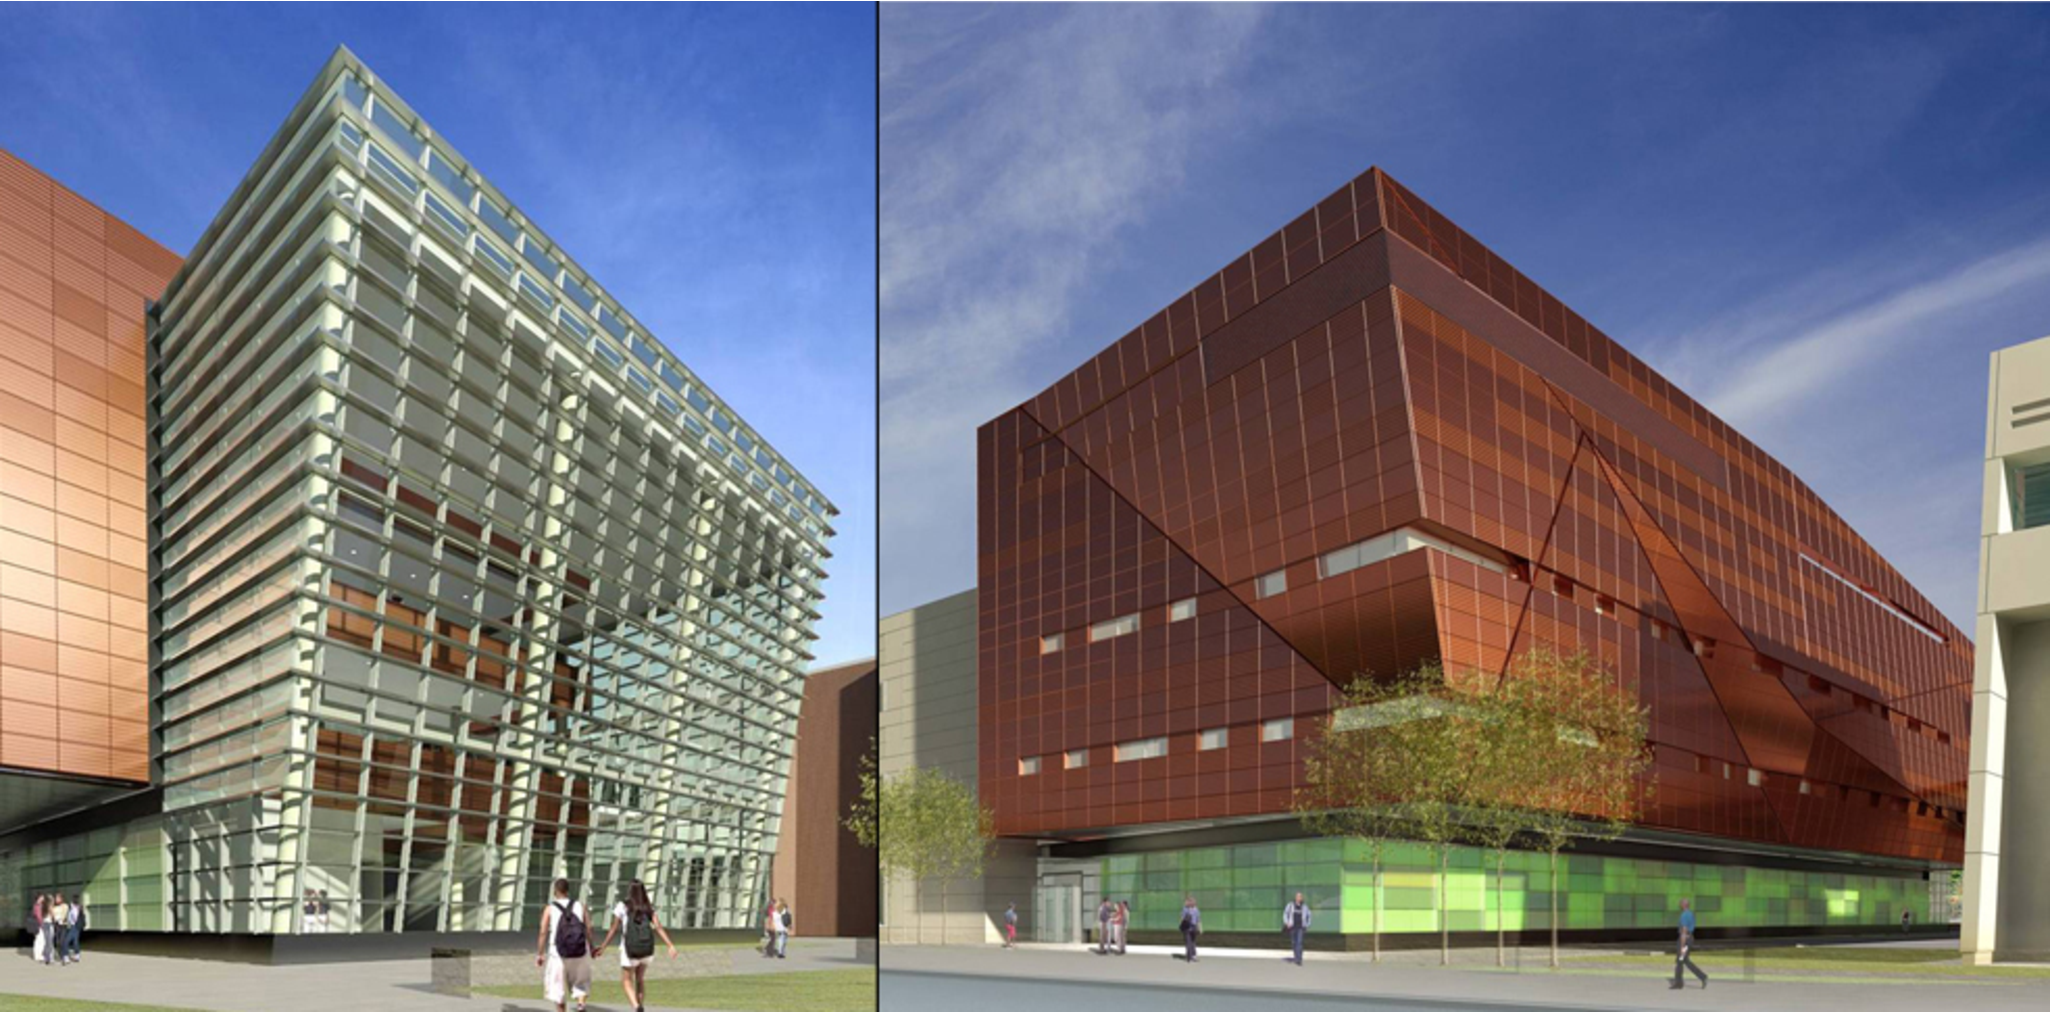
\includegraphics[width=\textwidth]{./figures/UBNewBuilding}
\caption{\textbf{New Davis UB Engineering Building}. The concept scheme shows the
SW elevation of the new \$75M Davis engineering building, scheduled to open in
summer 2011. (Image \copyright~Perkins Will.)}
\label{figure-newbuilding}
\end{figure}

\section{Facilities}

% 03 Feb 2011 : GWA : Standard departmental boilerplate.
%
% General research facilities include more than 200 i386 servers, x86\_64
% servers, SPARC-servers, PCs, and thin-client workstations. Available systems
% include three Dell Dimensions, thirty-four Dell Optiplexes, eight Dell
% PowerEdges, one Dell Precision, one Sun 5220, one Sun Blade 100, one Sun
% Blade 1000, one Sun Fire 280R, two Sun Fire V20Zs, more than 100 Sun Ray thin
% client terminals, and two Sun Ultra-60s. These systems are attached to a
% NetApp FAS2050A installed with 13 TB of disk space. Nine Dell Optiplex
% systems are configured as Linux and Windows student workstations. Laser
% printing resources are readily available. 

% 06 Dec 2010 : GWA : Use relevant descriptors.
%
%\textbf{\textsc{Laboratory:}}
%\textbf{\textsc{Clinical:}}
%\textbf{\textsc{Animal:}}
%\textbf{\textsc{Computer:}}
%\textbf{\textsc{Office:}}
%\textbf{\textsc{Other:}}

\section{Major Equipment}

% 03 Feb 2011 : GWA : Standard departmental boilerplate.
%
% Program-specific research facilities include 59 dedicated research systems.
% The Computer-Assisted Diagnostics Interventions Lab includes 23 systems, of
% which 18 members comprise a compute cluster connected to a 10 TB (installed)
% data storage device. The CyberInfrastructure Lab includes a 14-node compute
% cluster connected to a 15 TB (installed) data storage device. The
% Bioinformatics, Database, Data Mining, and Multimedia Group includes Dell and
% HP Oracle, MySQL, and compute servers. The Vision and Perceptual Machines Lab
% include two Apple Xserves. The 13 TB (installed) departmental
% network-attached storage device provides disk space for general and specific
% research projects.
